% L9c simulated annealing schematic: the loss from the gradient descent
% schematic (Fig-GD-Schematic), with a local minimum theta_2 and a lower
% minimum theta_1. Started at theta_3, simulated annealing moves downhill to
% theta_2, where gradient descent stops. At a high temperature it accepts an
% uphill move toward the hump and then moves downhill to theta_1. At a low
% temperature it rejects a large uphill move away from theta_1.
%
% Drawn on October 19, 2026 with the gradient descent schematic's curve,
% palette, and notation, so the two figures can be compared directly.
%
% The curve is the same four cubic Bezier segments. The states on it were
% computed from the same control points:
%   A: segment 1 at t = 0.6 -> (0.826, 2.799)
%   B: segment 2 at t = 0.8 -> (2.525, 2.882)
%   C: segment 3 at t = 0.5 -> (4.125, 1.800)
%   R: segment 4 at t = 0.8 -> (8.266, 2.512), the rejected candidate
% Each move is an arc above the curve from one state to the next.
%
% Math uses the standard TeX fonts (no unicode-math), so \theta renders as the
% same plain theta the notebook's math shows.
%
% The notebook SVG carries a dark palette added by theme_svg.py; keep new
% colors in that script's mapping when changing the palette here.
\documentclass[tikz,border=4pt]{standalone}
\usepackage[no-math]{fontspec}
\IfFontExistsTF{Arial}{\setsansfont{Arial}}{\setsansfont{TeX Gyre Heros}}
\renewcommand{\familydefault}{\sfdefault}
\usepackage{amsmath,amssymb}
\usetikzlibrary{arrows.meta,calc}

% Ink and the blue, red, and gray point colors match the gradient descent
% schematic; orange marks the accepted uphill move.
\definecolor{vnink}{HTML}{202124}
\definecolor{gdblue}{HTML}{0091FF}
\definecolor{gdred}{HTML}{E02020}
\definecolor{gdgray}{HTML}{6D7278}
\definecolor{saorange}{HTML}{F08C00}

\begin{document}
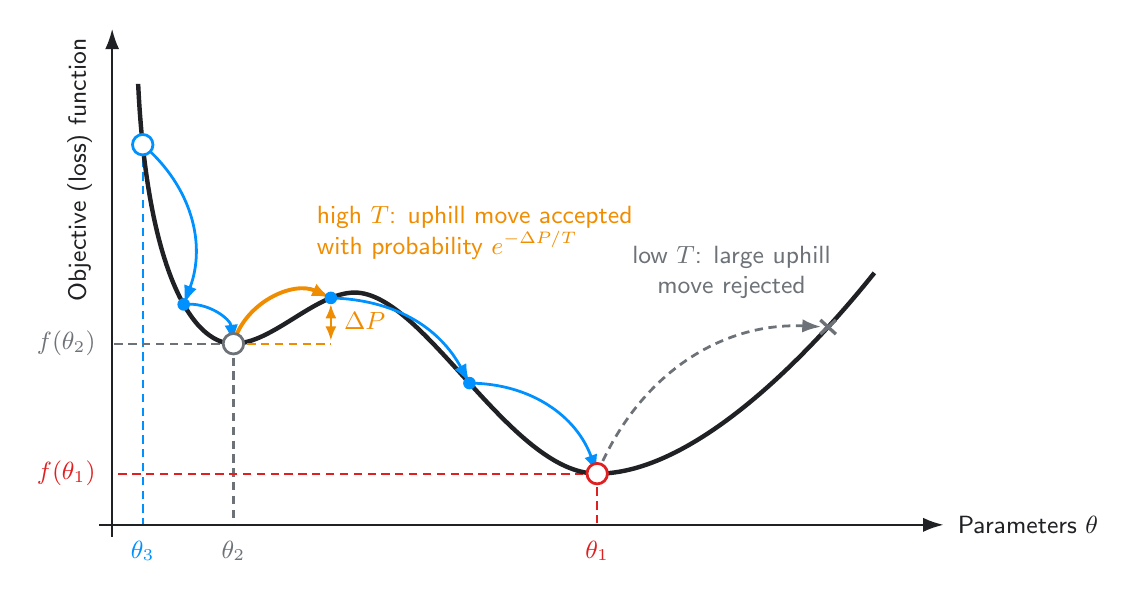
\begin{tikzpicture}[x=1.1cm, y=1cm, font=\sffamily\small, text=vnink,
    axis/.style={draw=vnink, line width=0.8pt, -{Latex[length=2.6mm, width=1.8mm]}},
    loss/.style={draw=vnink, line width=1.6pt},
    drop/.style={line width=0.8pt, dash pattern=on 3pt off 2pt},
    move/.style={line width=1.0pt, -{Latex[length=2.4mm, width=1.7mm]}},
    pt/.style={circle, fill=white, line width=1.0pt, inner sep=0pt, minimum size=2.6mm},
    state/.style={circle, fill=gdblue, inner sep=0pt, minimum size=1.6mm},
  ]
  % start point, minima, and the states along the run
  \coordinate (t3) at (0.353, 4.828);
  \coordinate (t2) at (1.40, 2.30);
  \coordinate (t1) at (5.60, 0.65);
  \coordinate (A) at (0.826, 2.799);
  \coordinate (B) at (2.525, 2.882);
  \coordinate (C) at (4.125, 1.800);
  \coordinate (R) at (8.266, 2.512);

  % dashed guides to the axes, drawn first so everything else sits on top
  \draw[drop, gdblue] (t3) -- (t3 |- 0,0);
  \draw[drop, gdgray] (t2) -- (t2 |- 0,0);
  \draw[drop, gdgray] (t2) -- (0, 2.30);
  \draw[drop, gdred] (t1) -- (t1 |- 0,0);
  \draw[drop, gdred] (t1) -- (0, 0.65);

  % axes
  \draw[axis] (-0.15, 0) -- (9.6, 0);
  \draw[axis] (0, -0.15) -- (0, 6.3);
  \node[anchor=west] at (9.65, 0) {Parameters $\theta$};
  \node[rotate=90, anchor=south east] at (-0.12, 6.3) {Objective (loss) function};

  % loss curve
  \draw[loss] (0.30, 5.60) .. controls (0.40, 3.30) and (0.90, 2.30) .. (1.40, 2.30)
    .. controls (1.85, 2.30) and (2.35, 2.95) .. (2.80, 2.95)
    .. controls (3.60, 2.95) and (4.60, 0.65) .. (5.60, 0.65)
    .. controls (6.70, 0.65) and (8.00, 2.10) .. (8.80, 3.20);

  % rise of the accepted uphill move, from f(theta_2) up to the state B
  \draw[drop, saorange] (t2) -- (B |- t2);
  \draw[saorange, line width=0.8pt, {Latex[length=1.8mm, width=1.4mm]}-{Latex[length=1.8mm, width=1.4mm]}]
    ($(B |- t2) + (0, 0.04)$) -- ($(B) + (0, -0.08)$);
  \node[anchor=west, text=saorange] at ($(B |- t2)!0.5!(B) + (0.04, 0)$) {$\Delta P$};

  % downhill moves (accepted at every temperature)
  \draw[move, gdblue] (t3) to[bend left=35] (A);
  \draw[move, gdblue] (A) to[bend left=45] (t2);
  \draw[move, gdblue] (B) to[bend left=30] (C);
  \draw[move, gdblue] (C) to[bend left=35] (t1);

  % accepted uphill move at a high temperature
  \draw[move, saorange, line width=1.4pt] (t2) to[bend left=50] (B);
  \node[anchor=south west, text=saorange, align=left] at (2.25, 3.25)
    {high $T$: uphill move accepted\\ with probability $e^{-\Delta P/T}$};

  % rejected uphill move at a low temperature
  \draw[move, gdgray, dash pattern=on 3pt off 2pt, shorten >=2.5pt] (t1) to[bend left=35] (R);
  \draw[gdgray, line width=1.2pt] ($(R) + (-0.09, -0.09)$) -- ($(R) + (0.09, 0.09)$)
    ($(R) + (-0.09, 0.09)$) -- ($(R) + (0.09, -0.09)$);
  \node[anchor=south, text=gdgray, align=center] at (7.15, 2.75)
    {low $T$: large uphill\\ move rejected};

  % axis labels for the three points
  \node[anchor=north, text=gdblue] at (t3 |- 0,-0.08) {$\theta_{3}$};
  \node[anchor=north, text=gdgray] at (t2 |- 0,-0.08) {$\theta_{2}$};
  \node[anchor=north, text=gdred] at (t1 |- 0,-0.08) {$\theta_{1}$};
  \node[anchor=east, text=gdgray] at (-0.08, 2.30) {$f(\theta_{2})$};
  \node[anchor=east, text=gdred] at (-0.08, 0.65) {$f(\theta_{1})$};

  % states along the run, then the open markers last
  \node[state] at (A) {};
  \node[state] at (B) {};
  \node[state] at (C) {};
  \node[pt, draw=gdblue] at (t3) {};
  \node[pt, draw=gdgray] at (t2) {};
  \node[pt, draw=gdred] at (t1) {};
\end{tikzpicture}
\end{document}
